\documentclass{beamer}
% \usepackage{animate}
\usepackage{multimedia}
\usepackage[english,russian]{babel}

\usepackage{pgfpages}
\setbeameroption{show notes on second screen}
%https://tug.ctan.org/macros/latex/contrib/beamer/doc/beameruserguide.pdf

\usepackage[T2A]{fontenc}
\usepackage[utf8]{inputenc}

\setbeamertemplate{caption}[numbered]

\usetheme{CambridgeUS}
\usecolortheme{dolphin}


\title[Геометрические преобразования]{Геометрические преобразования}
\author[Быковских Д.А.]{Быковских Дмитрий Александрович}
\date{27.09.2025}

\begin{document}
	\begin{frame}
		\titlepage
	\end{frame}

	\section{Геометрические преобразования}

	\begin{frame}{Геометрические преобразования}
		Цель: овладеть математическим языком описания динамики и визуализации.

		Представленные техники можно применять на различных этапах графического конвейера, в частности, связанных с обработкой вершин.
	\end{frame}

	\begin{frame}{Геометрические преобразования}
				
		Геометрическое преобразование --- отображение $f:R^n \to R^{n^{*}}$ $n$-мерного пространства прообраза в $n^{*}$-мерное пространство образа.

		Другой вариант записи:	
		$
			P^{*}=f(P)
			,
		$
		где 
		$P^{*} \in R^{n^{*}}$;
		$P \in R^n $.
		
		Виды преобразований:
		\begin{enumerate}
			\item Аффинные (affinity, $P^{*} = P  A+B$)
				\begin{enumerate}
					\item Линейные однородные ($B = [0]$)
					\begin{enumerate}
						\item Вырожденные (проективные, $\det{A} = 0$)
						\item Невырожденные ($\det{A}\neq 0$)
					\end{enumerate}
				\end{enumerate}
			\item Другие (например, $P^{*}=A P^2+B P+ C$ или отражение в кривом зеркале)
		\end{enumerate}

		\note{

		Аффинное преобразование (линейное неоднородное)

		\[
			\begin{bmatrix}
				p_x^{*} \\
				p_y^{*} \\
				p_z^{*} \\
			\end{bmatrix}^T
			=
			\begin{bmatrix}
				p_x \\
				p_y \\
				p_z
			\end{bmatrix}^T
			\begin{bmatrix}
				a_{0,0} & a_{0,1} & a_{0,2}  \\
				a_{1,0} & a_{1,1} & a_{1,2}  \\
				a_{2,0} & a_{2,1} & a_{2,2}  \\
			\end{bmatrix}
			+
			\begin{bmatrix}
				b_0 \\
				b_1 \\
				b_2
			\end{bmatrix}^T
		\]

		или с точки зрения размеров матриц
		\[
			(P^{*T})_{1,3}
			=(P^T)_{1,3} \times A_{3,3}+(B^T)_{1,3} 
			=(P^TA)_{1,3}+B_{1,3}^T 
			\]

		или тоже самое

		\[
			\begin{bmatrix}
				p_x^{*} \\
				p_y^{*} \\
				p_z^{*} \\
			\end{bmatrix}
			=
			\begin{bmatrix}
				a_{0,0} & a_{0,1} & a_{0,2}  \\
				a_{1,0} & a_{1,1} & a_{1,2}  \\
				a_{2,0} & a_{2,1} & a_{2,2}  \\
			\end{bmatrix}^T
			\begin{bmatrix}
				p_x \\
				p_y \\
				p_z \\
			\end{bmatrix}
			+
			\begin{bmatrix}
				b_0 \\
				b_1 \\
				b_2 \\
			\end{bmatrix}
		\]

		Если быть до конца точным, то какой-то из двух результатов нужно транспонировать.
		}
	\end{frame}

	\section{Трехмерные преобразования}

	\begin{frame}{Трехмерные преобразования}{3D tranformations}

		С помощью аффинных преобразований можно выполнять
		\begin{enumerate}
			\item масштабирование (scaling);
			\item вращение (rotation);
			\item перемещение (translation);
			\item сдвиг (shear).
		\end{enumerate}
		
		\centering{
		В компьютерной графике используются линейные (однородные) преобразования
		}
		\[
			\begin{bmatrix}
				p_x^{*} \\
				p_y^{*} \\
				p_z^{*} \\
				1
			\end{bmatrix}^T
			=
			\begin{bmatrix}
				p_x \\
				p_y \\
				p_z \\
				1
			\end{bmatrix}^T
			\begin{bmatrix}
				m_{0,0} & m_{0,1} & m_{0,2} & m_{0,3}  \\
				m_{1,0} & m_{1,1} & m_{1,2} & m_{1,3}  \\
				m_{2,0} & m_{2,1} & m_{2,2} & m_{2,3}  \\
				m_{3,0} & m_{3,1} & m_{3,2} & m_{3,3}  \\
			\end{bmatrix}
		\]
		\note{
			Почему вдруг матрицы стали размером $4 \times 4$?
			
			Откуда взялись 1? Почему не 0?
			\[
				\begin{bmatrix}
					p_x^{*} \\
					p_y^{*} \\
					p_z^{*} \\
					1		\\
				\end{bmatrix}^T
				=
				\begin{bmatrix}
					p_x \\
					p_y \\
					p_z \\
					1		\\
				\end{bmatrix}^T
				\begin{bmatrix}
						a_{0,0} & a_{0,1} & a_{0,2} & 0  \\
						a_{1,0} & a_{1,1} & a_{1,2} & 0  \\
						a_{2,0} & a_{2,1} & a_{2,2} & 0  \\
						b_{1}   & b_{2} 	& b_{3} 	& 1  \\
				\end{bmatrix}
			\]

			или кратко
			\[
				P^{*T}
				=
				P^T
				\begin{bmatrix}
					A & [0]  \\
					B & 1 \\
				\end{bmatrix}
			\]
			
			Какие коэффициенты необходимо изменить, чтобы добиться желаемого результата?
		}
	\end{frame}

	\begin{frame}{Масштабирование}{Scaling}
		
		Такое преобразование можно описать в виде системы уравнений
		
		\[
			\begin{cases}
				p_x^{*} = p_x s_x \\
				p_y^{*} = p_y s_y \\
				p_z^{*} = p_z s_z \\
			\end{cases}
		\]

		Тогда матрица масштабирования имеет вид:
		\[
			M_s = 
			\begin{bmatrix}
				s_x & 0 & 0 & 0  \\
				0 & s_y & 0 & 0  \\
				0 & 0 & s_z & 0  \\
				0 & 0 & 0 & 1 \\
			\end{bmatrix}
		\]
		
		\note{
			
			Если $s_i > 1$, то такое преобразование называется расширением.

			Если $0< s_i < 1$, то такое преобразование называется сжатием.
			
			Примечание:

			В случае, когда $s_i < 0$, такое преобразование называется отражением.
		}
	\end{frame}

	\begin{frame}{Перемещение}{Translation}
		
		Такое преобразование можно описать в виде системы уравнений
		
		\[
			\begin{cases}
				p_x^{*} = p_x + t_x \\
				p_y^{*} = p_y + t_y \\
				p_z^{*} = p_z + t_z \\
			\end{cases}
		\]

		Тогда матрица смещения имеет вид:
		\[
			M_t = 
			\begin{bmatrix}
				1 & 0 & 0 & 0  \\
				0 & 1 & 0 & 0  \\
				0 & 0 & 1 & 0  \\
				t_x & t_y & t_z & 1 \\
			\end{bmatrix}
		\]
		
		\note{}
	\end{frame}


	\begin{frame}{Вращение (Поворот)}{Rotation}
		
		Рассмотрим поворот в двумерной системе координат.

		\begin{center}
			Переход из полярной системы координат в декартовую
		\end{center} 



		\begin{columns}
			\begin{column}{0.5\textwidth}
				Пусть координаты точки $p$
				\[
					\begin{cases}
						p_x = r \cos \phi \\
						p_y = r \sin \phi \\
					\end{cases}
				\]

				А координаты точки $p^*$
				\[
					\begin{cases}
						p_x^* = r \cos (\phi + \theta) \\
						p_y^* = r \sin (\phi + \theta) \\
					\end{cases}
				\]
			\end{column}
			\begin{column}{0.5\textwidth}

				\begin{figure} 
						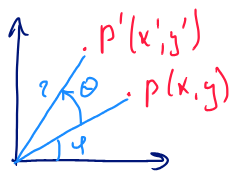
\includegraphics[width=0.6\textwidth]{images/rotation.png}
					\caption{Схема поворота}
				\end{figure}

			\end{column}
		\end{columns}



		В результате получаем следующую матрицу
		\[
			M_r(\theta) =
			\begin{bmatrix}
				\cos \theta & \sin \theta \\
				-\sin \theta & \cos \theta  \\
			\end{bmatrix}
		\]

		\note{
			\[
				\begin{cases}
					p_x^* = r (\cos \phi \cos \theta - \sin \phi \sin \theta) \\
					p_y^* = r ( \cos \phi \sin \theta + \sin \phi \cos \theta) \\
				\end{cases}
			\]

			\[
				\begin{cases}
					p_x^* = (r \cos \phi) \cos \theta - (r \sin \phi) \sin \theta \\
					p_y^* = (r \cos \phi) \sin \theta + (r \sin \phi) \cos \theta \\
				\end{cases}
			\]

			\[
				\begin{cases}
					p_x^* = p_x \cos \theta - p_y \sin \theta \\
					p_y^* = p_x \sin \theta + p_y \cos \theta \\
				\end{cases}
			\]

			\[
				\begin{bmatrix}
					p_x^* \\
					p_y^* \\
				\end{bmatrix}^T
			 =
			 \begin{bmatrix}
				p_x \\
				p_y \\
			\end{bmatrix}^T
			\begin{bmatrix}
				\cos \theta & \sin \theta \\
				-\sin \theta & \cos \theta  \\
			\end{bmatrix}
		\]
	
		}
	\end{frame}

	\begin{frame}{Вращение (Поворот)}{Rotation}
		Матрица вращения относительно оси $z$ на угол $\alpha$ против часовой стрелки

		\[
			M_r (\alpha) = 
			\begin{bmatrix}
				\cos \alpha & \sin \alpha & 0 & 0  \\
				-\sin \alpha & \cos \alpha & 0 & 0  \\
				0 & 0 & 1 & 0  \\
				0 & 0 & 0 & 1 \\
			\end{bmatrix}
		\]


		\note{
			Матрица вращения относительно оси $y$ на угол $\beta$ против часовой стрелки

			\[
				M_r (\beta) = 
				\begin{bmatrix}
					\cos \beta & 0 & - \sin \beta & 0  \\
					0 & 1 & 0 & 0  \\
					\sin \beta & 0 & \cos \beta & 0  \\
					0 & 0 & 0 & 1 \\
				\end{bmatrix}
			\]
	
	
			Матрица вращения относительно оси $x$ на угол $\gamma$ против часовой стрелки
	
			\[
				M_r (\gamma) = 
				\begin{bmatrix}
					1 & 0 & 0 & 0  \\
					0 & \cos \gamma & \sin \gamma & 0  \\
					0 & - \sin \gamma & \cos \gamma & 0  \\
					0 & 0 & 0 & 1 \\
				\end{bmatrix}
			\]
		
		
		Такие углы поворота вокруг осей называются углами Эйлера.}

	\end{frame}

	\begin{frame}{Сдвиг (Скос)}{Shear}
		% https://en.wikipedia.org/wiki/Simple_shear

		В трёхмерном пространстве сдвиг остаётся аффинной трансформацией, искажающей форму объекта, но сохраняющей объём. 
		Каждая координата может «сдвигаться» пропорционально остальным двум. 

		Такое преобразование можно описать в виде системы уравнений
		
		\[
			\begin{cases}
				p_x^{*} = p_x + sh_{xy}\,p_y + sh_{xz}\,p_z \\
				p_y^{*} = sh_{yx}\,p_x + p_y + sh_{yz}\,p_z \\
				p_z^{*} = sh_{zx}\,p_x + sh_{zy}\,p_y + p_z \\
			\end{cases},
		\]
		где
		$sh_{xy}$ --- сдвиг по X пропорционально Y;
		$sh_{xz}$ --- сдвиг по X пропорционально Z;
		$sh_{yx}$ --- сдвиг по Y пропорционально X;
		$sh_{yz}$ --- сдвиг по Y пропорционально Z;
		$sh_{zx}$ --- сдвиг по Z пропорционально X;
		$sh_{zy}$ --- сдвиг по Z пропорционально Y.
			
		\note{
			Тогда матрица сдвига (скоса) имеет вид:
			\[
				M_{sh} = 
				\begin{bmatrix}
					1 & sh_{yx} & sh_{zx} & 0 \\
					sh_{xy} & 1 & sh_{zy} & 0 \\
					sh_{xz} & sh_{yz} & 1 & 0 \\
					0 & 0 & 0 & 1
				\end{bmatrix}
			\]


			Свойства операции сдвига:
			\begin{enumerate}
				% \item 
				% Коэффициенты сдвига создают деформацию формы без изменения длин базовых векторов, смещая точки пропорционально их координатам.
				\item 
				Искажение формы, например, плоские грани превращаются в параллелограммы, а куб становится параллелепипедом;
				\item 
				Сохранение объёма, т.е. определитель матрицы остается тем же самым;
				\item 
				Сохранение параллельности, т.е. прямые, параллельные базовым осям, остаются прямыми, но меняют угол.
			\end{enumerate}
		}
	\end{frame}

	\begin{frame}{Последовательность преобразований}

		Замечание 1.

		Если, например, необходимо повернуть какой-либо произвольный объект вдоль какой-либо оси.

		\[
			P^* = P (M_t^{-1} M_r M_t)
		\]
		

		Замечание 2.

		Следующие преобразования эквивалентны:
		
		\[
			P^* = P (M_s M_r M_t)
		\]
		\[
			(P^*)^T = (P M_s M_r M_t)^T
		\]
		\[
			(P^*)^T = (M_s M_r M_t)^T P^T
		\]
		\[
			(P^*)^T = M_t^T M_r^T M_s^T P^T
		\]

		\note{
			\footnotesize
		Существующие реализации:

		\begin{enumerate}
			\item 
			(GPU stage) GLSL (OpenGL Shading Language) - это язык, используемый OpenGL (синтаксис основан на C) для запуска программ на графическом процессоре, называемых шейдерами, назначение которых вам известно. 
			GLSL предоставляет расширенные возможности для работы с векторами и матрицами по двум причинам:
			\begin{enumerate} \footnotesize
				\item 
				Отсутствует возможность загружать и использовать библиотеки.
				\item
				Программирование графики очень тесно связано с математическими преобразованиями.
			\end{enumerate}
			
			\item 
			(CPU stage) GLM (OpenGL Mathematics) - это библиотека C++, используемая для расширения математических возможностей с помощью функций и типов, которые обычно используются в графическом программировании.

			Причина, по которой GLM использует OpenGL в своем названии, заключается в том, что он был создан с учетом программирования графики (другими словами, создан для OpenGL).
		\end{enumerate}
		
		}
	\end{frame}

	\section{Кватернионы}

	\begin{frame}{Gimbal lock}

		При повороте внутренней рамки (второй) на 90 градусов механизм теряет своё основное свойство — хранить одно из направлений в трехмерном пространстве, т.е. происходит «складывание рамок».
		
			\begin{figure} 
				\href{https://youtu.be/zc8b2Jo7mno?feature=shared&t=79}{
					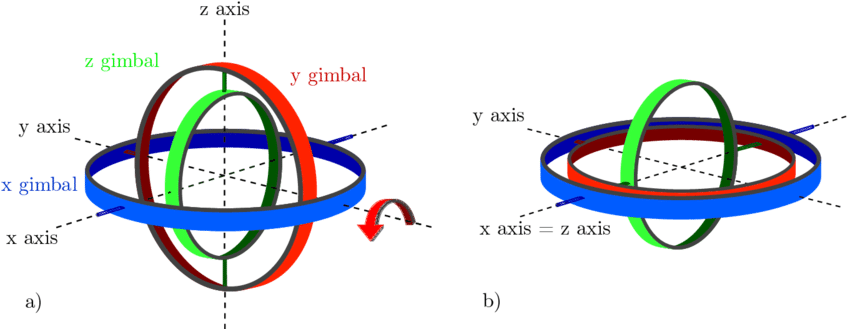
\includegraphics[width=0.8\textwidth]{images/llustrates-the-principle-of-gimbal-lock.png}}
				\caption{Возникновение проблемы при параметризации положения углового положения объекта}
			\end{figure}

		
		\note
		{

			Поскольку объект с одной закреплённой точкой имеет три степени свободы, то для параметризации, вообще говоря, достаточно задать три параметра. 
			
			Наиболее часто, но не всегда, в качестве таких параметров выбираются эйлеровы углы. 
			При этом существует такое положение объекта, при котором невозможно однозначно определить эйлеровы углы.

			Проблема возникает, если при последовательных поворотах объекта на эйлеровы углы, выполнить второй поворот на 90 градусов.

			Решение заключается в другом способе поворота объекта на нужный угол с помощью кватернионов.
		}

	
	\end{frame}


	\begin{frame}{Кватернионы} {Quaternions}
		
		Кватернионы --- система гиперкомплексных чисел.

		\[
		q = (s, v) = s + i x + j y + k z
		,
		\]
		где 
		$s$ --- действительная часть;
		$v = (x,y,z)$ --- вектор трехмерного пространства;
		$i, j, k$ --- мнимые единицы.

		\begin{table}
			\caption{\label{tab:quternion_times} Умножение базисных кватернионов}
			\begin{center}
				\begin{tabular}{|c|c|c|c|}
					\hline
					$\times$ & $i$ & $j$ & $k$ \\
					\hline
					$i$ & $-1$ & $k$ & $-j$ \\
					\hline
					$j$ & $-k$ & $-1$ & $i$ \\
					\hline
					$k$ & $j$ & $-i$ & $-1$ \\
					\hline
				\end{tabular}
			\end{center}
		\end{table}

		
		
		\note{
			Кватернионы были предложены Гамильтоном (1805 -- 1865) в 1843 г.

			Операции над кватернионами
			\begin{enumerate}
				\item Сложение
				\[
					q_1 + q_2 = (s_1+s_2, v_1+ v_2).
				\]
				\item Умножение
				\[
					q_1 \cdot q_2 
					= (s_1, v_1) (s_2, v_2) 
					= (s_1 s_2 - v_1 \cdot v_2, s_1 v_2 + s_2 v_1 + v_1 \times v_2)
					,
				\]
					где скалярное произведение
				\[
					v_1 \cdot v_2 =
					-( x_1 x_2 + y_1 y_2 + z_1 z_2)
					;
				\]
				векторное произведение
				\[
					\begin{vmatrix}
						i & j & k \\
						x_1 & y_1 & z_1 \\
						x_2 & y_2 & z_2 \\
					\end{vmatrix}
					=
					i (y_1 z_2 - z_1 y_2) 
					- j (x_1 z_2 - z_1 x_2)
					+ k (x_1 y_2 - y_1 x_2)
					.
				\]
			\end{enumerate}
		}


	\end{frame}

	\begin{frame}{Вращение вокруг произвольной оси} {Quaternions}
		
		Для того чтобы выполнить вращение вокруг произвольной оси $u=(u_x,u_y,u_z)$ на угол $\theta$ некоторой точки $p(p_x,p_y,p_z)$, необходимо выполнить следующую последовательность действий:

		\begin{enumerate}
			\item Подставить координаты точки $p$ 
			в мнимую часть кватерниона:
			$q_p = (0,p)$;
			
			\item После нормирования вектора $u$ преобразовать ось вращения $u$ и угол $\theta$ в виде кватерниона:
			$q_r = (\cos \theta / 2, u \sin \theta / 2)$;
			
			\item Вычислить по формуле $q_p^{*}=q_r q_p q_r^{-1}$, причем 
			$q_p^{*} = (s^{*},p^{*}) = s^*+i p_x^*+jp_y^*+kp_z^*$; 
			
			\item Извлечь результат из мнимой части кватерниона $q_p^{*} = (s^{*},p^{*})$.
			Таким образом,
			 $p^* = (p_x^*, p_y^*, p_z^*)$.
		\end{enumerate}
		
		\note{
			Примчения:

			Если $\theta > 0$ то вращение выполняется по часовой стрелке.

			Нормирование вектора $u$:

			\[
				u = \biggl( \frac{u_x}{|u|},\frac{u_y}{|u|},\frac{u_z}{|u|} \biggr),
			\]
			где $|u| = \sqrt{u_x^2+u_y^2+u_z^2}$ --- длина вектора $u$.

			Сопряжение кватерниона $q$:

			Для кватерниона $q$ сопряженным называется кватернион 
			\[
				q^{-1} = (s, -v).
			\]
		}
	\end{frame}

\end{document}
